Para el diseño de este controlador se eligió $k_p = 3,5$ resultante de una relación de compromiso entre el margen de fase y la rapidez del controlador. En la Figura \ref{fig:bode_p} se puede observar el diagrama de Bode a lazo abierto con sus respectivos márgenes de fase y ganancia.

\begin{figure}[H]
  \centering
  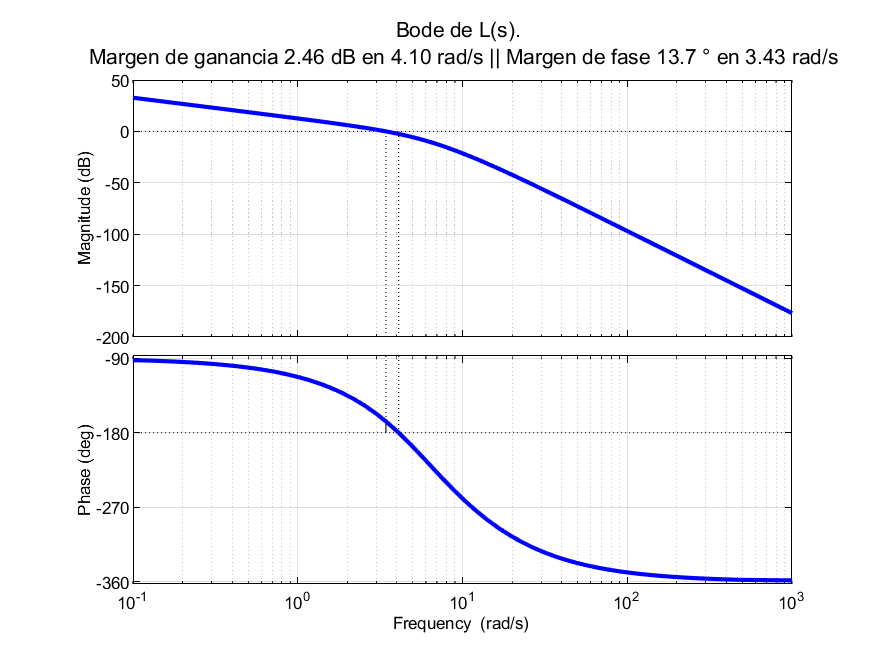
\includegraphics[width=0.75\textwidth]{img/P/Proporcional-Bode de L.png}
  \caption{Diagrama de Bode de $L(s)$.}
  \label{fig:bode_p}
\end{figure}

En las Figuras \ref{fig:impulso_p} y \ref{fig:escalon_p} se observan las respuestas al impulso y al escalón a lazo abierto medidas y simuladas, respectivamente.

\begin{figure}[H]
  \centering
  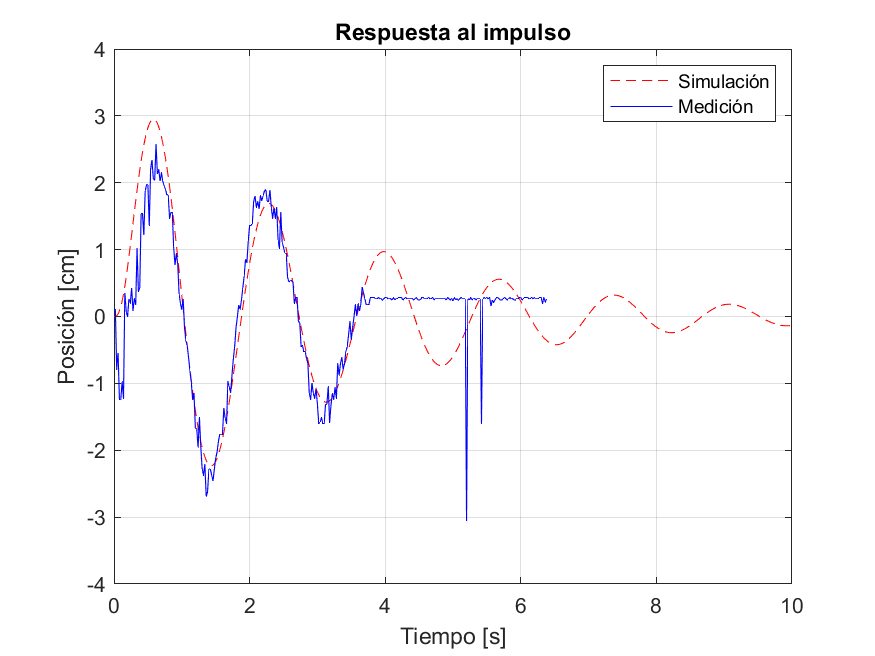
\includegraphics[width=0.75\textwidth]{img/P/proporcional-respuesta al impulso.png}
  \caption{Respuesta al impulso de $T(s)$.}
  \label{fig:impulso_p}
\end{figure}

\begin{figure}[H]
  \centering
  
\includegraphics[width=0.75\textwidth]{img/P/proporcional-respuesta al escalón.png}
  \caption{Respuesta al escalón de $T(s)$.}
  \label{fig:escalon_p}
\end{figure}

La estabilización cerca de la referencia, mas no en ella se debe al rozamiento intrínseco de la barra y ruedas del carrito. Esto se corregirá con una componente integradora en el controlador.